%
%
%
\subsection{Impulsively accelerated flat plate}
\label{accelerated_flat_plate.subsec}
%
 To demonstrate the capability of the present method for unsteady flow,
 the solution of an impulsively accelerated flat plate in the laminar regime
 is presented. This example is also known as Stokes first problem
 and an analytical solution for incompressible flow is available
 (Schlichting \citeyearNP{Schlichting}, Mattioli \citeyearNP{Mattioli:1}).
 This analytical solution shows that the time dependent
 solution collapses to a single solution of nondimensional velocity versus
 the similarity parameter $\eta$ defined as

%
\beq
  \eta = \frac{y}{2\sqrt{\nu t}}
  \label{stokes_first1.eq}
\eeq
%
 where $y$ is the normal distance from the flat plate, $\nu$ is the kinematic
 viscosity and $t$ is the physical time. The analytical solution take the
 simple form

%
\beq
  \frac{u}{u_\infty} = {\tt erf}\left(\eta\right)
  \label{stokes_first2.eq}
\eeq
%
 where $\tt erf$ represents the error function (Schlichting \citeyearNP{Schlichting}).
%
\begin{figure}
 \begin{center}
  \begin{tabular}{c}
    \subfigure[Velocity profiles]
       {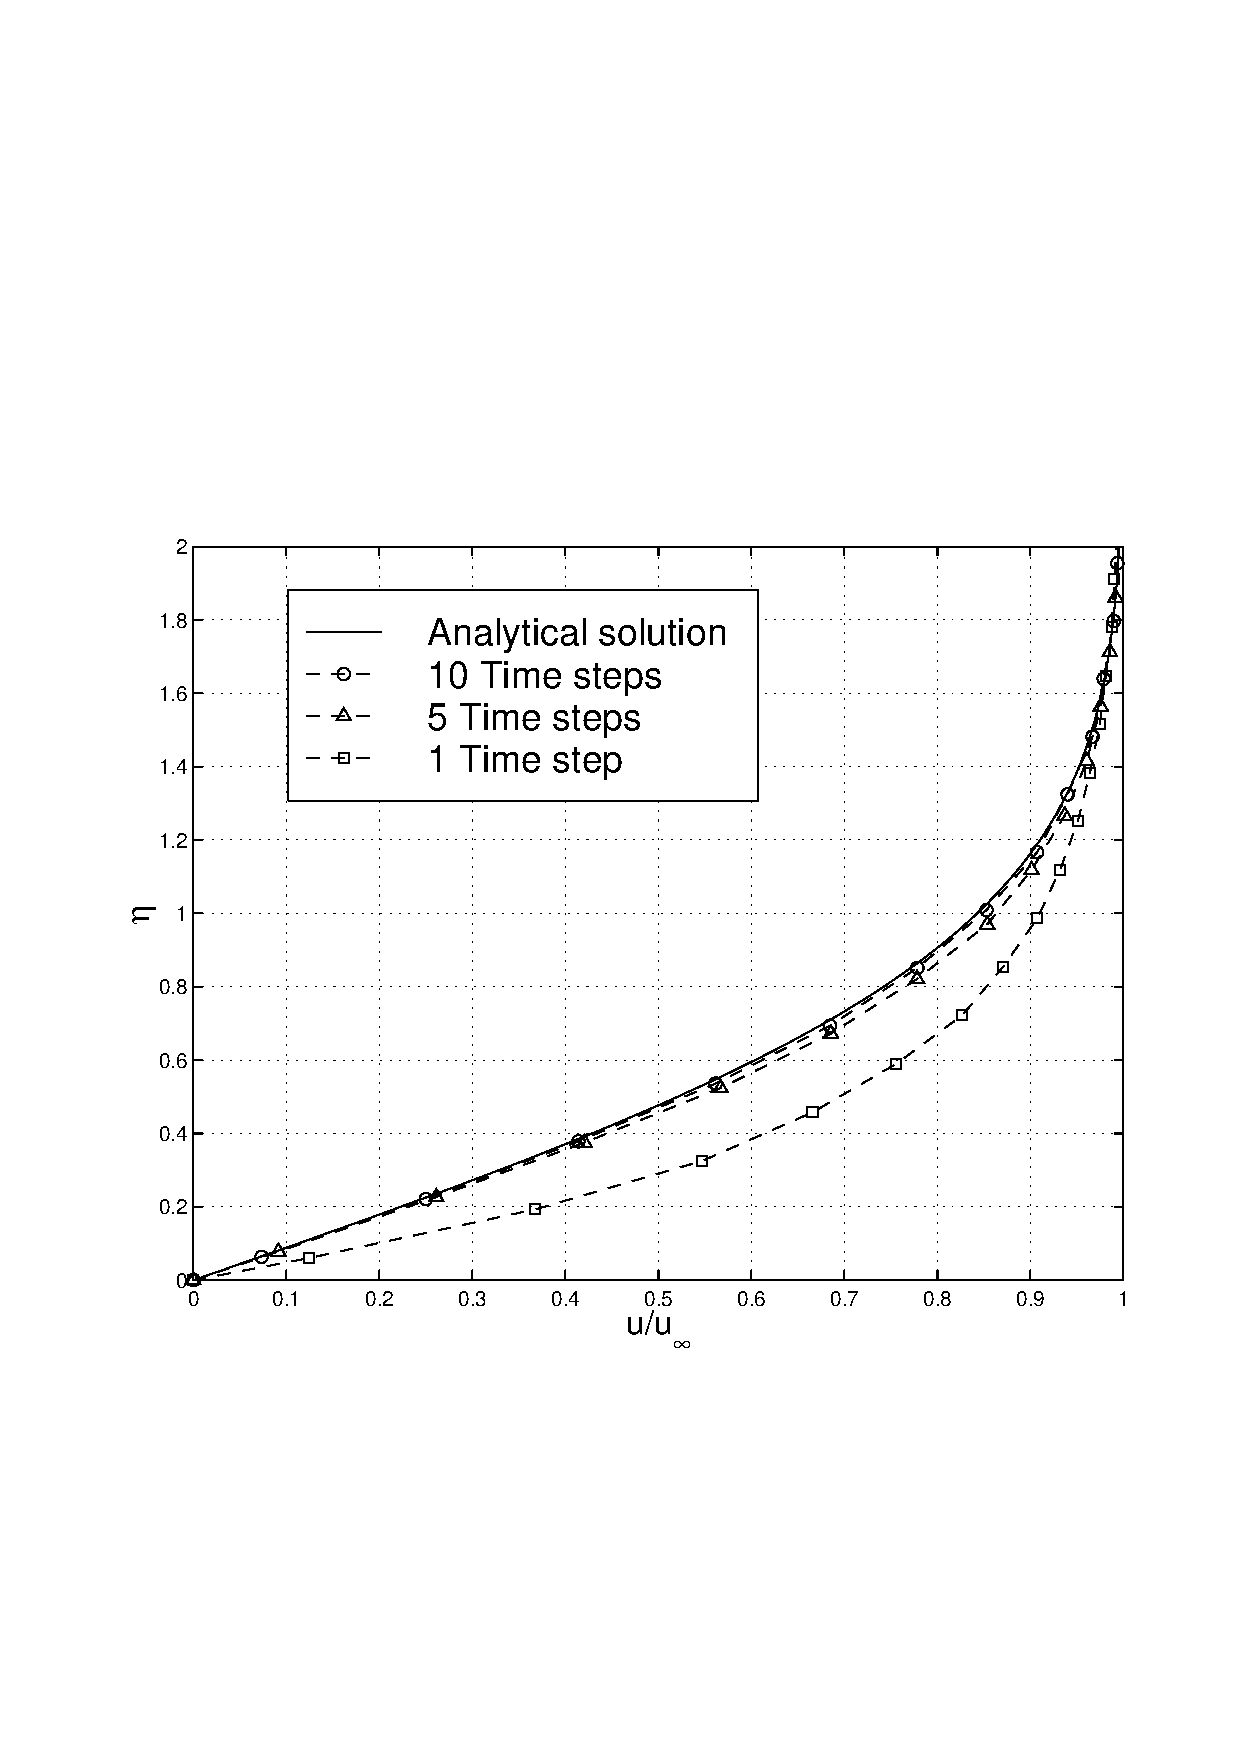
\includegraphics[width=110mm,clip=t]{CHAP_NONLIN/FIGURE/flat_sol.pdf}}
        \\
    \subfigure[Convergence history]
       {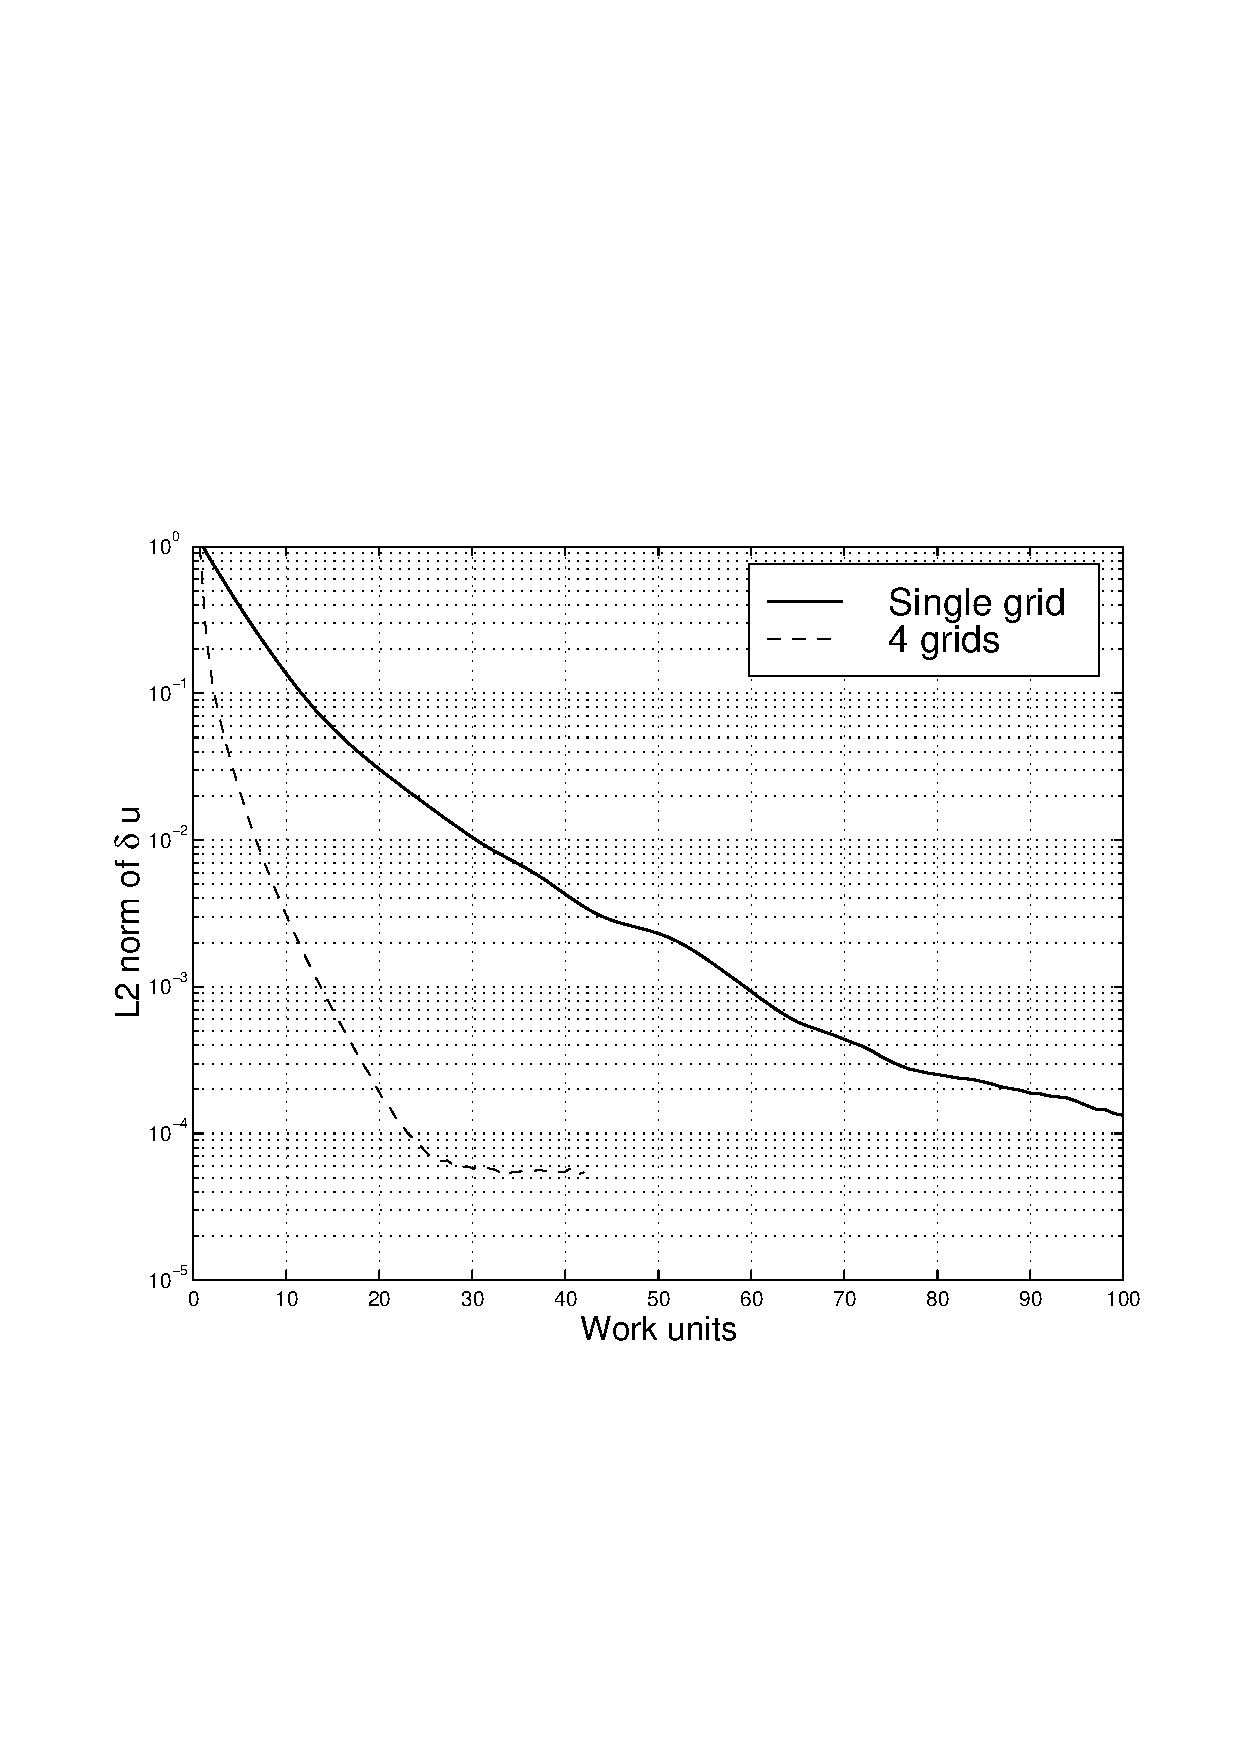
\includegraphics[width=110mm,clip=t]{CHAP_NONLIN/FIGURE/flat_res.pdf}}
  \end{tabular}
 \end{center}
 \vspace{-8mm}
 \caption{Impulsively started flat plate. $M_\infty = 0.2$, $Re_\infty = 40,000$.
          Velocity profiles and residual history}
 \label{flat_impul.fig}
\end{figure}

 Three calculations were performed with the present method with 1, 5 and 10
 physical time steps to reach the same physical time $t = 0.001\ sec$.
 The maximum ratio between the physical and pseudo time step, $\Delta t/\Delta\tau$,
 was of around 17,000 for the case where a single time step was used to reached
 $t = 0.001\ sec$. Fig. \ref{flat_impul.fig}a shows the comparison between
 the numerical and analytical solutions. As expected, the smaller the physical time
 step, the better the agreement.
 If one used an explicit method to calculate the unsteady flow at the same physical
 time level, than it should have performed around 15,000 time steps using
 a CFL number of 1.5. For the case of 5 time step the convergence of
 (\ref{Dual_time_stepping_3.eq}) for a given time level was obtained with $\approx 15$
 W multigrid cycles using four grids. In terms of CPU time this means
 that with 5 time steps the present method was $\approx 120$ times faster than
 an explicit Runge-Kutta integration method.

 Fig. \ref{flat_impul.fig}b shows the comparison of the
 residual within a given physical time step, using a single grid and a four grids
 W-type cycle. As one would expected, the convergece to a new physical time level
 improves if more the one grid are used. However such improvement does not
 compare with the one obtained for steady-state computations.
 Convergence histories similar to the one
 shown in Fig. \ref{flat_impul.fig}b represents the best result
 obtained for unsteady flows.
